\documentclass{acm_proc_article-sp}
\usepackage{xspace}
\usepackage{hyperref}

\begin{document}

\title{LifeScope: A Multimodal Mobile Time Tracking Application}

\numberofauthors{3}
\author{
% 1st. author
\alignauthor
Luca Foschini\\
       \affaddr{University of California, Santa Barbara}\\
       \email{foschini@cs.ucsb.edu}
% 2nd. author
\alignauthor
Danny Iland\\
       \affaddr{University of California, Santa Barbara}\\
       \email{iland@cs.ucsb.edu}
% 3rd. author
\alignauthor 
Ian Whitfield\\
       \affaddr{University of California, Santa Barbara}\\
       \email{ianwhitfield@cs.ucsb.edu}
}

\def\LS{{\tt LifeScope}\xspace}

\maketitle
\begin{abstract}
In this paper, we present \LS, an Android app that tracks and identifies the daily activities of a handheld device user.
\LS harnesses input from a variety of sensors as well as cloud service APIs to determine what activity is being performed by the user at any given time. Detected activities can then be summarized on a time and geographic scale, as chosen by the user.

In what follows, we describe the architecture of \LS, and discuss our design choices. Finally, we present an evaluation of \LS in terms of accuracy of the activity detection and battery usage.
\end{abstract}

% A category with the (minimum) three required fields
\category{H.5}{Information Systems}{INFORMATION INTERFACES AND PRESENTATION}
\terms{Mobile computing, context-aware, multimodal interaction}

\section{Introduction}
The modern smartphone provides the possibility to connect to a wide array of sensors, some of them on-board, and some of them standalone. This ultimately enables sensor-rich computing on the phone, which in turns opens up new possibility of interaction with the user. The modern smartphone also has continuous, high-speed internet access. By using sensor-fusion for the smartphone's local sensing capabilities and by interfacing with various cloud services, the smartphone can act as a gateway to monitor the user's daily activity.
These increased monitoring capabilities have unlocked the possibility of ``self knowledge through numbers'', to put it like the recently founded movement Quantified Self~\cite{quantified:self}. That means applying analytics to your daily activity to gain knowledge about your life, with the goal of ultimately improving it.
However, the Quantified Self is only a milestone in the ongoing tendency towards tight integration of computing devices with human beings. After detecting activities and analyzing them, smartphones provide a gateway to perform actions in response to activities. This means closing the loop and have the smartphone to affect our daily life by performing actions (e.g., sending emails, texts, playing a notification sound, etc.) in response to the recognized user activities.

%%%%%%%%%%%%%%%%%%%%%%%%%%%%%%%%%%%%%%%%%%%%%%%%%%%%%%%%%%%%%%%

\section{Related Work}
There has been increased interest in the pervasive computing community around "context monitoring" and "context recognition" for mobile devices, particularly smartphones. Context recognition applications are able to identify a person's activity at a particular point in time~\cite{fahy2004cass}. A further development in the field of context recognition is the idea of context monitoring~\cite{lee2012mobicon} which involves executing complex, multi-step operations and correlating the output of different sensors.

While the research community has mainly focused on defining a middleware platform to provide context information to the application layer in order to centralize and coordinate access to the shared sensors, such systems are usually experimental and not yet freely available.
An exception to the rule is The {\tt funf} Open Sensing Framework~\cite{funf}  from the MIT Media Lab. Funf is freely available, open source, and ready to use. {\tt Funf} provides a common layer abstraction on the device sensors. The management of sensors is centralized and allows multiple applications to interact with the same sensor without causing conflicts or dramatically increase usage. Funf is designed to continuously collect data and log it to the device's internal flash memory or an SD card. Its data sources include any of the standard Android sensors (e.g. accelerometer, gyroscope, compass); operating system-level information, such as which applications are currently open; and data from other applications on the phone, including browser bookmarks, user contacts, and recent searches. To protect the user's privacy, sensitive data (such as a recent search string) is passed through a one-way hash function. Funf will automatically download updated configuration files (which sources to collect from, and at what rate) and periodically upload recorded data through the device's internet connection. This makes funf ideal for widespread data collection, where a large pool of devices can be centrally managed by a small team of researchers.

To conclude the review of related work, we discuss {\tt on\{X\}} a recent product developed at Microsoft~\cite{onx}. {\tt on\{X\}} provides a framework to program actions to be executed automatically by a smartphone when conditions on sensors are met. Example are ``Launch the music app when I am walking'' or ``Launch calendar when I arrive at work''. 
Microsoft {\tt on\{X\}} can be viewed as the evolution of early apps that would change basic behavior of the phone based on the context, one example being Android Locale~\cite{android:locale}, which mutes the phone depending on its location. 

The development of context-aware applications has just begun. Both {\tt funf} and {\tt on{X}}  have been released in the last months and the natural expectation to have is that a lot more has yet to come in the realm of context aware applications.


%%%%%%%%%%%%%%%%%%%%%%%%%%%%%%%%%%%%%%%%%%%%%%%%%%%%%%%%%%%%%%%

\section{Implementation Overview}

\LS builds on the idea that human activities are usually strongly localized. For this reason, \LS tries to detect activities only when a transition in location is detected, i.e., a user arrives at or leaves a place. While this model does not support activities that span multiple places, we believe that it adequately models the majority of use cases and greatly simplifies the rest of our implementation. 

In general, \LS works as follows. When a transition in location is detected (departure from or arrival at a place) events corresponding to sensor readings collected since the previous location transition are analyzed to identify activities. The principle is sketched in Figure~\ref{figure:principle}

\begin{figure}
\begin{center}
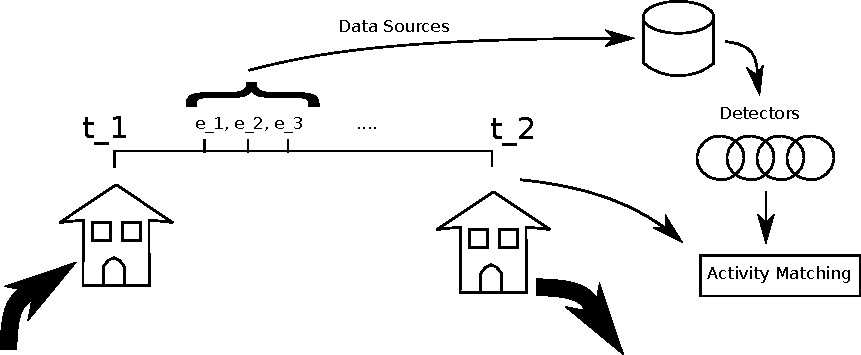
\includegraphics[width=3in]{logic}
\caption{
Between two location transition (arriving home and leaving home) events $e_1, \dots, e_n$ are stored in a database by Data Sources. Various data sources perform the task of polling sensors and storing timestamped reading in a database. When a location transition ``leaving from home'' is detected, the detection engine queries the database to retrieve events stored by the Data Sources during the time interval $[t_1, t_2]$. Events are then matched with rules to detect activities. 
}
\label{figure:principle}
\end{center}
\end{figure}


Therefore, our approach can then be broken down into two main components: identifying places that a user travels to and then, once at a place, identifying the activity performed.

\subsection {Action Recognition}
We now describe how activities are detected by \LS. First, the user defines an activity to be matched as a list of conditions that have all to be satisfied on sensors, in the form of {\tt ittt} rules\cite{ittt}, detected by what we call Detectors.

\paragraph{Detectors}  Detectors are the core component of our activity recognition system, each of which activates in response to a specific, predefined condition. 
The user groups configured instances of Detectors into actions with descriptive titles such as "working on CS 290". When all the detectors for an action are active when the user is at a location, it is determined that the user was performing that action at that location. The Detectors are backed by Data Sources, which maintain databases of events that may cause a Detector to activate. A Data Source may store its data locally, or may be acting as a proxy for a cloud service API such as Google Calendar. 

\paragraph{Example} A possible activity to be recognized could be described by:
\begin{quote}{\it If} I'm on campus, my phone is plugged in, and I have an event about 290I on my calendar, {\it then} I must be working with my team on the 290I project.\end{quote}. This means that if in the time interval between two consecutive location transitions (e.g., arriving at a place, then leaving it) a location detector, along with a calendar and a plugged\_in detectors are all triggered, the action ``Working on the 290I project'' is detected.


\subsection {Location Management}

Since activities take place at specific locations an important first step was to be able to accurately determine a user's currnedot location and detect when they move to a new location. For this we decided to use two approaches. We use Alohar, a third-party API, which uses Wi-Fi SSIDs (and their associated signal strengths) combined with GPS to accurately and continuously record a phone's position. Alohar runs as a service in the background, and launches on startup. Alohar also performs filtering and analysis of this location data, in order to provide a rich API, which can be easily queried. A query for locations visited in a specific time range results in a list of Alohar UserStays, which consist of a centroid latitude and longitude, a time of arrival and departure, and several candidate Place objects, each with a name, address, and category. We map these UserStays in the Locations tab, and display the best guess Place data.

It is important to note that Alohar UserStays are created only when multiple location readings indicate a stable centroid latitude and longitude. In our experiments, it took Alohar 5-10 minutes to create a UserStay after arriving at an indoor location with many nearby access points. The accuracy of start times and end times appears to be good. [TODO(Danny): Will elaborate] The UserStays centroid/lat long was on average X meters away from the true centroid as manually recorded, and X away from the lat/long identified by Location Service... charts and such.

Since we wish to allow arbitrary location-based detectors, we also register a listener for Google's Location Service, and log the current latitude and longitude at 30 second intervals. This allows detectors to set location triggers, and locations to be recognized even if they are ephemeral in nature, and would not create an Alohar User Stay. 



\subsection {Application Architecture}
Due to its widespread adoption and rich application API (especially for background activity), we decided to implement LifeScope as a user-installable application (``App'') for the Android smartphone operating system.

Internally, our application is structured as a pair of always-running Service components with a number of standalone Activity components that connect to them. The first Service component hosts the currently enabled Detectors and Data Sources. It allows Data Sources to collect data from device sensors and cloud APIs even when the user is not actively using the application. Client Activity components may connect to this Service to register new actions (which contain Detector instances), or determine which of the registered actions has been performed at a given location.

The second Service contains the Alohar and Google location tracking systems and, as with the first service, allows them to continue running in the background and log events when the user transitions to a new location.

Events from both the Data Sources and location trackers are stored in SQLite databases for simple querying from Detectors and, if desired, custom queries by the user from another SQLite client.

\begin{figure}
\begin{center}
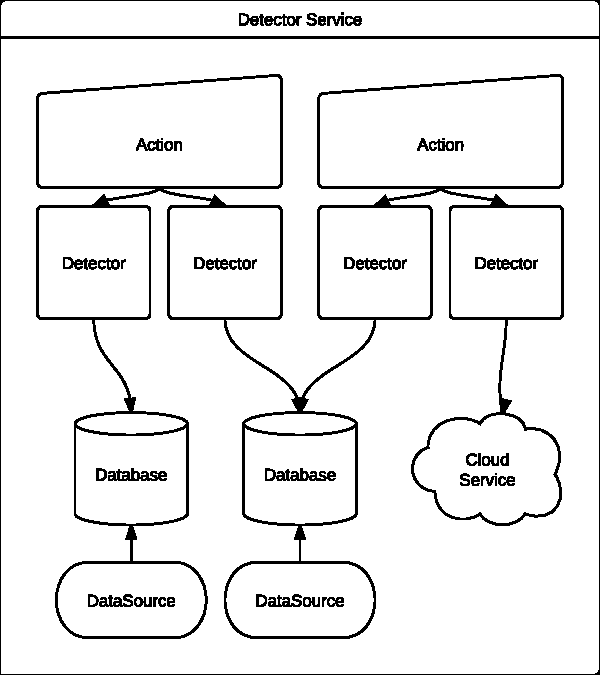
\includegraphics[width=3in]{arch}
\caption{
Architecture of the Detector Service, which stores registered Actions and Detectors and allows the Data Sources to run in the background collecting data.
}
\label{figure:voice}
\end{center}
\end{figure}

\subsection{Detectors Implemented}

We implemented the following detectors:
\begin{description}
\item[Calendar] configured with a string $s$, when queried for timerange $[t_1,t_2]$ tries to find a match of $s$ in the activity of the user's google calendar in that timerange.
\item[Workout] when queried for timerange $[t_1,t_2]$ computes the moving average of the accelerometer values in int $[t_1,t_2]$ to assess substantial activity which could indicate the user is working out. 
\item[Proximity / Plugged\_in] when queried for timerange $[t_1,t_2]$ return if the device has been in proximity (resp. plugged in) in the interval $[t_1,t_2]$. The data source for these detectors samples the sensor state every 1 minute.
\end{description}

Our extensible architecture allows to easily add new detectors.


\subsection {User Interface}
The user interface was designed to follow Android best-practices and features a number of different interaction modes. As is typical for a modern smartphone application, basic interaction with the application is performed with a simple tapping interface. 

A major component of our application is the interactive map view, which shows places the user has visited (and stayed at for a period of at least 5 minutes). The map view supports a richer set of touch interaction modes with dragging to pan the map, pinching to zoom the map and, after first selecting a menu option, dragging to adjust the position of existing place markers.

As entering text is often a cumbersome task on smartphones without actual keyboards all text entry fields within the application have been extended with a voice input button, Figure \ref{figure:voice}.

\begin{figure}
\begin{center}
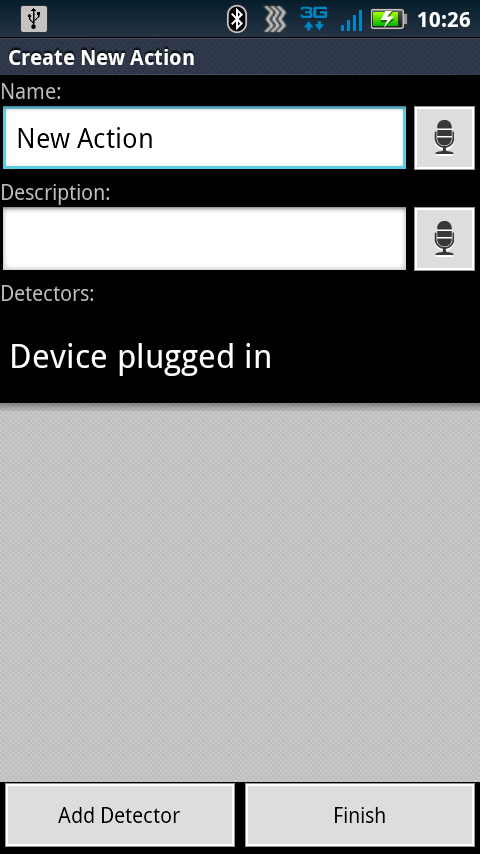
\includegraphics[height=2.5in]{voiceinput}
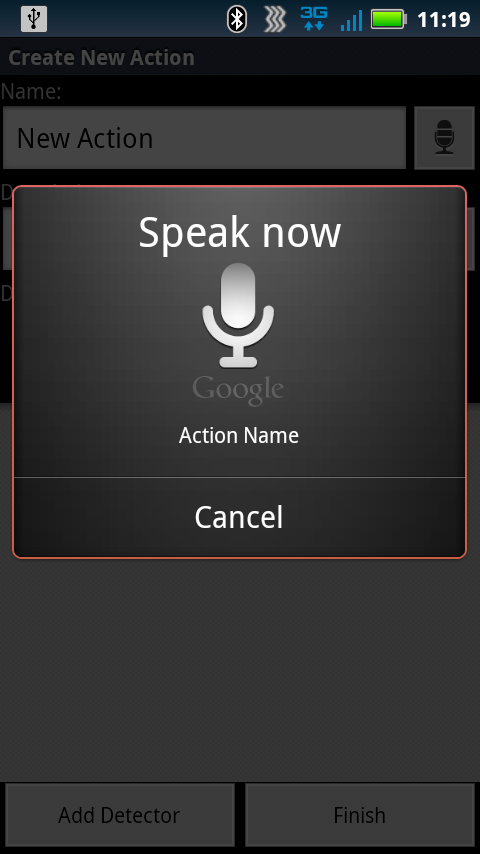
\includegraphics[height=2.5in]{voiceinput2}
\caption{
Creating a new action. All text fields are extended with a voice input button with a microphone icon. Tapping a voice input button records, recognizes, and then populates the corresponding text field with the user's speech. 
}
\label{figure:voice}
\end{center}
\end{figure}

\begin{figure}
\begin{center}
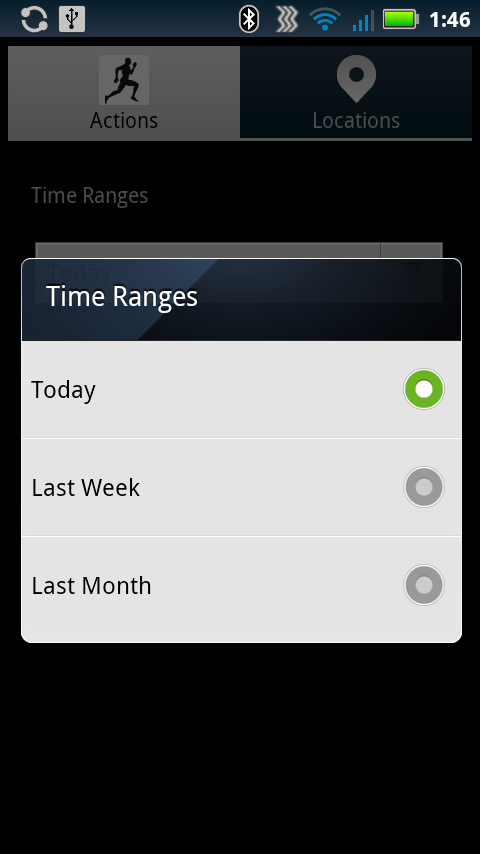
\includegraphics[height=2.5in]{ranges}
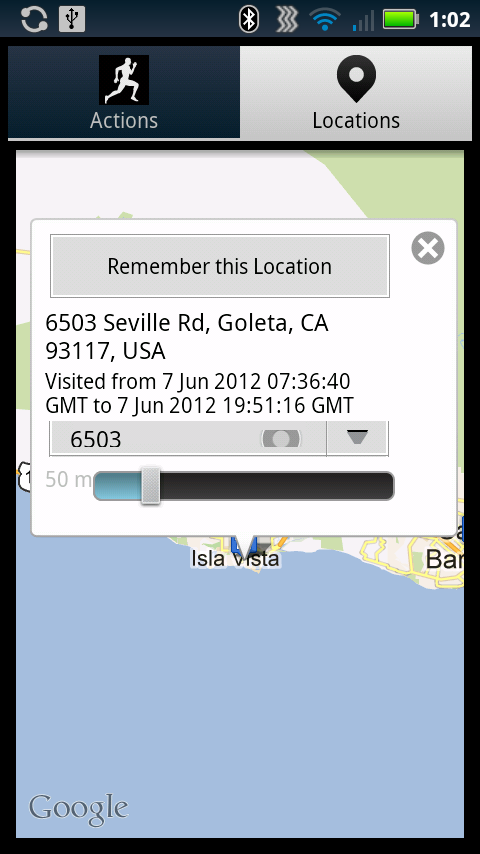
\includegraphics[height=2.5in]{map1}
\caption{
The two main views of the application. On the left, the activity summary. A spinner allows selecting a time range on which activities are aggregated and reported. On the right, the location summary. Locations where activities have been identified are highlighted and the user can interact with them.
}
\label{figure:voice}
\end{center}
\end{figure}

%%%%%%%%%%%%%%%%%%%%%%%%%%%%%%%%%%%%%%%%%%%%%%%%%%%%%%%%%%%%%%%

\section{Assessment}

It is certainly hard to evaluate the effectiveness of a system such as \LS without an in-depth user study. Therefore, we follow the example of~\cite{lee2012mobicon} and focus on evaluating specific aspects of the inner workings of \LS, with an emphasis on power consumption.

\subsection{Power Consumption}
An important design consideration for smartphone applications is their impact on battery life. If an application consumes so much power that the device prematurely runs out of power, the user will likely uninstall the application. Mobile context monitoring is an inherently expensive activity, in terms of power usage. The GPS and WiFi radios must remain on for accurate position estimates, and CPU cycles are required for analyzing data samples taken from the device's on-board sensors. For the application to build a complete model of the user's activities, it must remain running in the background and even when the phone is asleep. 

To minimize power draw \LS disables Data Sources that are not currently required by any registered Detectors. For example, if there are no detectors that need readings from the accelerometer sensor, its Data Source will not be activated and no samples will be read from the accelerometer. When the user adds an action containing a Detector that requires information from the accelerometer Data Source, it will be started automatically. Thus, the exact power usage of the application depends on how the user has configured it.

To understand how different detectors affect power usage, we performed a series of experiments. In each experiment one Data Source was enabled, and then the phone was left in its sleep state for a fixed period of time. The battery level was measured before and after each experiment to determine the effect of each Data Source on the device's battery life.

\subsection{Location Accuracy}
One fundamental subsystem of \LS is composed by the Alohar and Google location tracking systems. They notify \LS of a location transition, therefore their accuracy in determining the exact location is crucial. We measured the accuracy of \LS for [DANNY, FILL IN] for a set of known locations. We compared the geolocation returned by Alohar when being at one of the known locations to the geolocation available from Google Earth, to assess accuracy. 
We found that on average (N=5 locations) the error is 13m (standar deviation= 5.4m).


%%%%%%%%%%%%%%%%%%%%%%%%%%%%%%%%%%%%%%%%%%%%%%%%%%%%%%%%%%%%%%%

\section{Conclusions and Future Work}
In this paper we present \LS, an android app that allows users of a handheld device to track and analyze their daily activity. \LS leverages input from a variety of sensors to determine what activity is being currently performed by the user. \LS then provides methods to summarize all of the user's activities on a given timeframe or geographic area.
We evaluated the accuracy of sensor identification for the geographic location and the battery usage of the app. We found that the battery usage in the case \LS is set up to monitor a reasonable amount of activities is negligible. We also found that the location estimation, a task crucial for \LS, is quite precise.

\paragraph{Future Work} As far as the future work is concerned, we recognize that a system like \LS would benefit of many additional features if it were to be released to the general public. 
First, more detectors are needed to be able to describe a richer set of activities.
Second, a mechanism to guide and correct the detection of activities would be beneficial, for which the user can review or change the detected action. This is especially true if such a mechanism allowed the app to learn from the user feedback.
Finally, another possible improvement could be the ability to specify actions not only using {\tt ittt} rules, but by recording the sensor inputs while performing an activity to be recognized later, and then try to match such inputs to future sensor readings. Such a "record activity" feature is highly desirable to minimize user interaction, but it is hard to implement, as current research in activity identification still focus on identifying basic actions such as running/biking/driving ~\cite{mccallmacro}

%%%%%%%%%%%%%%%%%%%%%%%%%%%%%%%%%%%%%%%%%%%%%%%%%%%%%%%%%%%%%%%

\bibliographystyle{abbrv}
\bibliography{bibliography}  % sigproc.bib is the name of the Bibliography in this case

% That's all folks!
\end{document}
